\chapter{The Mattock Architecture}
This appendix tries to show the rough outlines of a possible future computer forensics framework that would built on the good parts and lessons learned from the Open Computer Forensics Architecture (OCFA), current day technological advancements, modern insights from the field of computer forensics and high-volume data processing, access control technologies and the concepts and sub-systems introduced in the MattockFS dissertation that this document was written as an appendix for. 
The idea of this appendix is to draw a rough outline of a possible, partially OCFA inspired framework using modern day information technology components and insights gained from years of OCFA usage and the analysis done on OCFA timing that was described in Appendix-A. A framework that, if completed, could fill the gap that in an academic sense was left by the discontinuation of OCFA development by the Dutch police. While this gap has been filled successfully for Dutch law enforcement by the Xiraf framework developed by the Netherlands Forensic Institute, and while on a smaller scale the framework provided by PyFlag and more notably the Sleuthkit Hadoop Framework have taken interesting steps, PyFlag, has not moved significantly beyond any of the same legacy implementation choices that OCFA made towards an architecture, to something more in sync with modern distributed computing insights. The Sleuthkit Hadoop Framework efforts on the other hand, like OCFA seem to have been abandoned. Neither architectures have addressed the basics of disk-cache efficiency as addressed in this paper. As far as a literature study has revealed, no open source frameworks that exists today has managed to provide the academic community with a framework suitable both for both small scale experiments and for the crucial experiments that work with a more sizeable lifelike data corpus and server cluster setup. Computer forensic research projects of the scale of for example the FIVES project that used OCFA at its core would hardly be possible today. 
This while OCFA in itself was actually never designed with an academic setting in mind. The framework described in this appendix
aims to first and foremost address the needs of computer forensic academic research, while keeping use as an alternate tool in cybercrime and other real world computer forensics investigations a serious option. 
While implementation of a full open source academic forensic framework with the required properties falls far outside of the scope of a single M.Sc research project, this appendix will provide the architectural outline of such a framework and will explain how MattockFS would play a pivotal role in the realization of such a framework. We shall address the base architectural design proposed in this appendix as \emph{The Mattock Computer Forensic Framework}. The idea of the naming stems from the naming of the carving tool scalpel. The idea is that while a tool the size of and with the precision of a scalpel is indispensable at any scale, if you want to scale up your investigations to the scale of an archeological dig, you will need bigger tools like a mattock. Its just a working title for the prospect architecture. Anyone picking up on this paper is invited to come up with a more suitable name for the resulting framework. 
\section{The OCFA architecture}
\begin{figure}
\centering
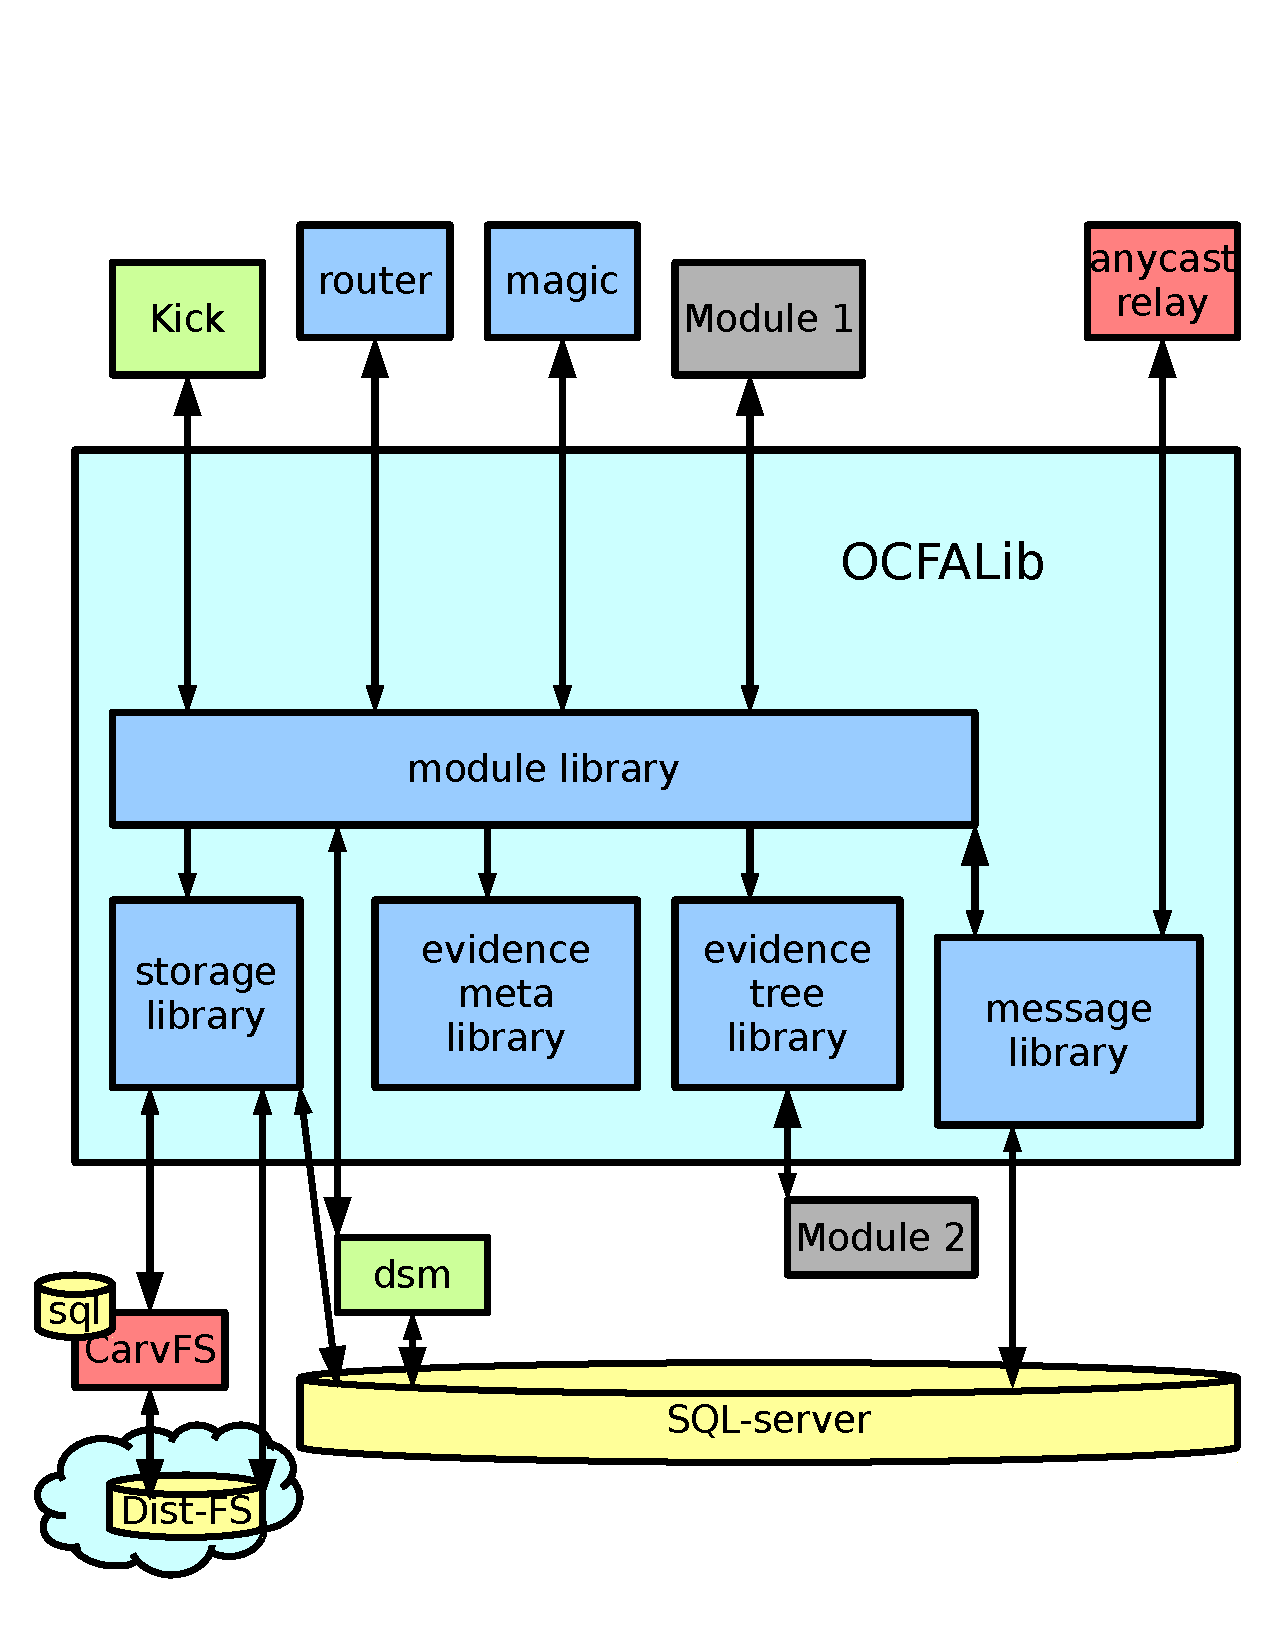
\includegraphics[width=100mm]{mattock/libraryview.pdf}
\caption{The base OCFA architecture}
\label{fig:FlowInOut}
\end{figure}
When we look at the OCFA architecture, at its core we can clearly identify fully custom build asynchronous messaging framework for processing modules that communicate with a small set of networking components that act to combine the modules into dynamic chains of tools that are applied to parts of the forensic evidence data. The use of commodity software components is mostly limited to the pervasive use of XML technology and a central relational database. We shall now have a look at some of the core components of the OCFA framework.
\subsection{The AnyCast Relay and Persistent Priority Queue}
At its basis, OCFA was a message passing concurrency based system. One known issue with message passing concurrency is the use of buffers. While message passing environment like the Erlang programming language and platform opt to put producing processes to sleep when buffers fill up, OCFA opted for a different approach. In OCFA, the message passing buffers were managed by on-disk persistent priority queues. These queues only contained referenced to in database large text objects. The persistent queues were meant and designed to be fully crash resistant. The priority queues had a special \emph{'never'} priority to hold messages that were observed to crash specific modules. This allowed modules to be restarted and to skip problematic data until a maintenance programmer would look at the problematic data and buggy module to fix the problem and re-submit the messages in the never queue for further processing. The AnyCast relay was built on top of the persistent priority queue. Every module connected to the AnyCast relay and registered as a consumer of a certain type (a module \emph{instance}) and would go into a message processing event loop asking the AnyCast relay for new jobs. When a module was done with a piece of evidence data, or when a module derived a sub entity from such data (for example an attachment as child entity of an e-mail message), the module would send a message to the AnyCast Relay addressed at a special process named the \emph{router}. The AnyCast would keep track of irresponsive and broken network connections and would play an important role in having stale or crashed modules restarted in a way not unlike what is common practice in Erlang based architectures. On such a detected crash, messages that were still pending a response would be put aside in the never queue to be looked at by a technician at a later point in time. In OCFA the AnyCast relay served as a single server for all modules, independent of the server these modules would run on.
\subsection{OcfaLib, a domain specific asynchronous framework}
While today NodeJS has mainstreamed the idea of a generic asynchronous framework, and while in other programming languages generic asynchronous frameworks such as Twisted for Python or Boost::asio for C++ have been available for quite a while, OCFA was first built long before such systems became mainstream. As a result, OCFA basically ended up building its own asynchronous processing framework. We could say that OcfaLib, the C++ OCFA library was a domain specific asynchronous framework for use with the AnyCast server. 
\subsection{The legacy Module API}
OCFA came with two quite distinct module Application Programming Interfaces (APIs). This fact was the result of chronology of development. The first version of OCFA came with a module API not much unlike that of the current day Sleuthkit framework. A module would get a file to process and could add meta data to that file, or, when it wanted to for example mark an extracted e-mail attachment as child entity, would submit that information to the framework. The API consisted of a module initialization part and a single method called 'processEvidence' that a module was supposed to overload. From within processEvidence the module could either add meta or submit a child entity with added meta date.
\subsection{The Tree-graph API}
After new modules got added to OCFA, the legacy module API was found to be lacking in the meta-data area. The problem was that a module deriving a tree of children would not be able to set meta-data for deeper child entities. Only level zero and level one meta data was possible. As a result, the more powerful tree-graph API was added. As porting old modules to the new API was considered a waste of precious development time, the old API was also still continued after the introduction of the new API.
\subsection{The legacy CAS storage}
OCFA in its initial release came with a Content Address Storage system for storing data entities. Data was created or, lacking CarvPath facilities, first copied to a temporary file and hashed during copy. Once the hash was fully calculated, the temporary file was either moved to a location derived directly from the hash of its content, or discarded if an entity with the same hash was already present in the repository. 
\subsection{CarvFS}
Later releases of OCFA were made compatible with the use of CarvFS for parts of the storage needs. CarvFS integration has however remained a bit of a hack. The storage sub-system of OCFA used physical symbolic links to CarvFS CarvPaths inside of its primarily CAS based storage system. This meant that for example when using a CarvPath aware Sleuthkit MMLS module, storage of a partition in the OCFA CAS storage system required the full partition to be read for hashing purposes before it could be symlinked in the storage subsystem.
\subsection{The meta-data based message router}
At the core of the OCFA architecture was the central meta-data based router. This XML technology based router would parse the meta-data that modules had gathered on a data entity and would based on an also XML-based rule-list determine the next hop in the tool-chain for that data entity. 
\subsection{The use of an SQL server}
There were two technologies that were pervasively used within OCFA. One XML we already discussed. The second one was a relational database. It was used by the storage subsystem, by the messaging subsystem, and finally by the meta-data storing data-store-module. In each of these uses, the use of an SQL database turned out to be a sub-optimal choice for a number of reasons. Some related to the creation of run-time performance bottlenecks and others related to the nature of the data structure and the nature of useful analysis-time queries on this data. More on this when we discuss the alternatives for Mattock.
\section{PyFlag}
\begin{figure}
\centering
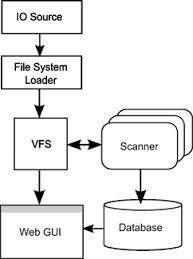
\includegraphics[width=50mm]{mattock/pyflag.jpg}
\caption{The base PyFlag architecture}
\label{fig:FlowInOut}
\end{figure}
Next to OCFA, the PyFlag framework deserves mention in this paper. While PyFlag has quite a different scope than OCFA it shares a lot of similarities too. Where OCFA is meant purely as a framework for computer forensics, PyFlag is a hybrid system that also addresses the field of network forensics. This hybrid approach makes that this framework would in a fundamental way be much more difficult to apply disk-cache related optimizations. It thus would be unfair to look at PyFlag purely from a large scale computer forensic data processing point of view in a comparative way. 
\section{The Sleuthkit Hadoop framework}
A more promising development was the Sleuthkit Hadoop framework. It aimed to combine The Sleuthkit with specific distributed technology. The technology proposed was a combination of the HDFS distributed file-system and the distributed NoSQL database HBASE, both part of the Hadoop technology stack. That is, a distributed file-system and NoSQL technology. We shall look in more detail at suitable NoSQL technology. While HBASE isn't a bad choice at the processing end, there are data structure and analysis concerns that would point to different NoSQL technology as potentially more suitable. Further, the \emph{initial read} performance of \emph{redundant} distributed storage might make looking closely at the performance/redundancy aspects for any distributed storage system. Today the concept of erasure encoding based distributed storage might provide an interesting middle ground between the two. Yet, taking a more NUMA or striping approach to scaling the storage for distributed computer forensic data processing might also proof an interesting alternative. 
\section{Non-open frameworks}
It is important to note that due to the closed nature of the frameworks involved, this paper does not look into some major and widely successful non-open forensic frameworks such as Xiraf or FTK Distributed Install. The scope of this appendix is limited to open tools and publications.
\section{Digital Evidence Bags}
So far we have been looking purely at scalability and performance of forensic architectures without considering other important new computer forensic insights. One conceptual idea that all current frameworks seem to discard are the key concept introduced with so called Sealed Digital Evidence Bags (S-DABs) by Bradley Schatz and Andrew Clark in 2006. While the details of S-DEBs fall outside of the scope of this appendix, one key aspect deserves special attention: The concept that both data and meta-data require a form of tamper-proofness. That is, once a piece of evidence data or meta-data is entered into the system, this (meta-)data should be considered to be logically immutable. We shall take this concept with us in our outlines for e next generation scalable framework.
\section{New insights}
Looking back at OCFA and other forensic frameworks, there are in retrospect important suboptimal choices that would be made differently if a framework like that was to be developed today. In this section we summarize a few important insights that arose from years long usage of OCFA, a survey of other open frameworks. A literature survey and the results of the timing analysis in the first appendix of this paper.
\begin{itemize}
\item \emph{A tree-graph API is essential} : While simpler API's can be useful for some trivial modules, all such modules could also work with a more generic tree graph API. Having just one generic tree-graph oriented API could facilitate a much wider range of modules and if the API is defined in asynchronous terms, the API could be portable to alternative architectures.
\item \emph{Leveraging asynchronous frameworks is essential} : OCFA implemented its own custom asynchronous framework and the part of the OCFA code-base involved with implementing that functionality was substantial. With current day asynchronous frameworks such as Boost::asio (C++), Twisted (Python) or NodeJS (JavaScript), the need for a custom built asynchronous framework has disappeared.
\item \emph{Evidence sealing, privilege separation and access control facilities are a must} : It is essential to limit the mutability time-span and scope to an absolute minimum. Both from an anti-forensics point of view, and from the point of view of the legal credibility of the integrity of the implemented forensic process.
\item \emph{Reducing disk-cache misses is essential for performance}: While many papers focus on CPU cycles being wasted by inefficient forensic processes, the truth is that much of the forensic process is IO rather than CPU constrained. As such, the fact that the same data \emph{will} get read multiple times should make clear that a disk-cache miss will impact throughput and that a forensic framework such as OCFA with a design that does not effectively mitigate disk-cache miss rates will suffer from throughput disk-cache-miss related IO bottlenecks.
\item \emph{Zero-storage carving is essential} : The process of locating, carving and validating files on disk images is complex and will either result in high false positive or high false negative counts. In the case of high false-positives, copy-out will result in massive needs for forensic archiving storage for derived entities. In the case of high false negatives essential data may be missed. Applying zero-storage carving facilities such as CarvFS will allow for a relatively low cost of false positives while minimizing the amount of additional storage required for processing.
\item \emph{Simple priorities don't really work} : While our research has shown that priority queuing as used in OCFA would be effective for homogeneously sized chunks of evidence data, not taking into account the size of the evidence entities and their likely disk-cache status in prioritizing has been shown to yield such poor results that the usefulness of priority queuing in such a way must be seriously questioned. 
\item \emph{Most current day forensic disk image formats are poorly suited for large-scale processing archives} : In large scale investigations encompassing dozens to hundreds of full-size disk images, the in-lab usage of the common computer forensic disk image storage formats (EFF \& AFF) have shown to be rather poorly suited due mostly to scalability issues of keeping hundreds of opened disk-image state-object open. Lacking a forensic-lab storage format for large archives of disk images, the use of simple sparse dd images currently seems to be better suited in a scalable lab environment than the direct usage of these formats. It would be good if future research would investigate the possibilities of archive friendly low system-footprint storage of a multitude of computer forensic data. 
\item \emph{Data migration should not be taken lightly} : While distributed file-systems or storage systems such as SNFS can facilitate in making evidence data available on many nodes, it is important to realize that accessing data from a different node will per definition result in a disk-cache miss on that node. It is suggested that data migration should prefer either the early out-of-cache migration of data that has not yet been fully cached by the originating module, or the migration of relatively small chunks of data targeted for relatively high-CPU processing on the other node. 
\item \emph{Relational (SQL) databases are a poor fit on most fronts} : In OCFA the Postgress SQL database was used for many things. In retrospect, certainly given the current day alternatives, these things would today all have better alternatives. First of all, the database usage for \emph{mutable} meta-data and for the storage and messaging subsystem together was a major performance bottleneck. Apart from the fact that in retrospect in-process mutable meta-data does not fit in with the S-DEB view of things, a relational database is a poor choice of technology for implementing either such meta-data \emph{document} storage or the extra indirections implemented within the storage and messaging subsystems. More than that though, the usage of an SQL database by the data storage module and the user interface have shown that many of the more advanced analysis's have had such shape and form that the database and queries would have been much better of having a more \emph{graph} oriented infrastructure. If we look at OCFA and than look at modern NoSQL technology, we see that parts of the SQL functionality had better be implemented without a database, some had better be implemented with a distributed \emph{key/value store} database, some with a \emph{document} database and some with a \emph{graph} database.  One thing all aspects of OCFA have in common is that SQL technology in todays technology landscape would be a sub-optimal choice at best. 
\item \emph{Kick-starting may not start at a server node} : In OCFA kick-starting took place from a server node. Before this could be done however, the EWF files had to be placed on an SNFS partition accessible to the server from a client through an SNFS connected file-server. Combine this with the need for converting EWF to dd or an other lab friendly format, the lack of a client-based EWF submitter led to massive disk write inefficiency. A kick-starting network client would need to be an essential component in a modern forensic framework.
\item \emph{Not all modules are alike} : Todays open source computer forensic frameworks treat modules as equal citizens. The reality however is that some modules such as a file-type module are so common in data processing that framework embedding would be justified, some modules such as simple carvers are used mostly on huge data files and are IO intensive while others like OCR work on relatively small data chunks and take up significant CPU resources. Treating all modules and all data as similar will inevitably lead to poor overall framework performance. 
\item \emph{Globally valid annotations are the key} : As each server in a forensic data processing cluster has its own disk cache, the concept of dividing the load between different nodes by distributing and redistributing to different nodes should be positively influenceable by allowing nodes to have a common communicable notion of the portions of the global investigation data they and other nodes likely still have in their cache. For this, a globally valid annotation for data chunks is essential CarvPath annotations could play a major role in this.
\item \emph{Meta-data serialization technology matters} : At the time that OCFA was devised, XML was the only logical choice for meta-data serialization. The XML technology stack though is far from being the most efficient serialization form for forensic meta data. While there are multiple papers proposing standardized XML formats for forensic meta-data exchange, the inefficiency and resource requirements of XML processing forms a major bottleneck in event-rich high throughput processing environments such as within a computer forensic framework. More efficient serialization options such as JSON, Protocol Buffers or Cap'n Proto should be seriously considered as alternative to XML. 
\item \emph{Hashing algorithm choice is essential} :  Traditionally MD5 and later also SHA1 have been used as hashing algorithms in digital forensics. From a cryptographic point of view, MD5 is now deprecated while SHA1 is in the process soon becoming deprecated. Many public and law-enforcement-only hash collections such as for example the Virusshare hash set or national child pornography hash sets are still distributed only with MD5 and/or SHA1 hashes. Others like the NIST NSRL are now supplemented with SHA256 hashes. While the later may sound like good news, there is an other important issue with SHA256 for use in a forensic framework: SHA256 may be significantly more secure as a hashing algorithm than SHA1 or MD5, it is also significantly more CPU intensive. So much so that it may undermine the whole concept of opportunistic hashing as presented in this paper. While today NIST still considers the use of SHA1 for purposes as defined in this paper as \emph{acceptable use}, we must consider the retroactive impact that a cryptographer testifying on behalf of the defense and questioning the continued use of (the no longer collision resistant) SHA1 in the forensic process may have a few years from now. It thus can be argued that moving forward to a non-deprecated secure hashing algorithm should be considered a priority. Given the CPU resource issues with SHA256, it is also of paramount significance that the algorithm we move forwards to should have at least reasonable resource requirements in its software implementation. A quick study into available secure hashing algorithms reveals a small family of secure hashing algorithms. SKEIN, BLAKE and BLAKE2 share properties that would make each of these secure hashing algorithms prime candidates for supplementing and eventually replacing SHA1 as primary hashing algorithm for computer forensics. In the next appendix we will make the case for one of these. The important insight here however is the notion that SHA1 is close to deprecation, SHA256 puts to much strains on resources in a high performance computer forensics setup and we need to pick a more suitable replacement.     
\end{itemize}
\section{A modernized OCFA inspired open-source architecture}
With the good parts from the old OCFA architecture combined with the new insights above, we can sketch the base outlines of a next generation message passing concurrency open computer forensic framework. Let us start out with a rough description of the changes from the OCFA architecture to our new Mattock architecture outline. The most obvious change can be seen in the dependencies. We no longer have a central SQL server dependency.  We see that the custom asynchronous framework gets replaced with a standard asynchronous framework. This could be boost::asio for C++ or for example twisted for the Python language. We see that file-type logic and meta-data router are no longer a separate module and network service but are now integrated in the base functionality for each module process. As in OCFA, a module instance runs in its own process as part of the asynchronous framework that it runs under. One module instance per async-framework process and possibly more module instances per module type if the server architecture and module type warrant multiple instances of the same module to be run on the same machine.  These could be CPU intensive modules on a server with a high amount of cores. 
We see that the number of module APIs reduced to just the tree-graph API.  The most obviously notable change however is the fact that there is no longer a direct dependency between generic modules and database technology. The SQL server has disappeared and has been replaced by other technology. The Data Store Module (DSM) maps the meta-data into some NoSQL database. This will most likely be a distributed graph-database or a distributed document-database (or possibly a hybrid combination of the two such as ArangoDb). Both data and now also meta-data are stored in a write-once way to the CarvFS replacement MattockFS that implements a subset of the S-DEB concept by means of privilege separation and immutability. The CarvFS long-path SQL database is replaced with a distributed key/value NoSQL database. While MattockFS should initially still run on something like SNFS, the use of a distributed file-system should be a potential way forward to further improve scalability. The AnyCast Relay functionality has mostly moved to a system bus like facility provided by the MattockFS filesystem, combined with a monitoring and load balancing mesh-up that connects the AnyCast functionality of all Mattock server nodes and will migrate jobs to other nodes when and only when the CPU needs for a job are expected to outweigh the cost of the page-cache miss on the peer node. One node per worker host. The kick-starting process is revised. EWF processing is moved to the client side of things. The client connects to a central kick balancer that will query all AnyCast monitors to find the right kick server to redirect the client to. 
\begin{figure}
\centering
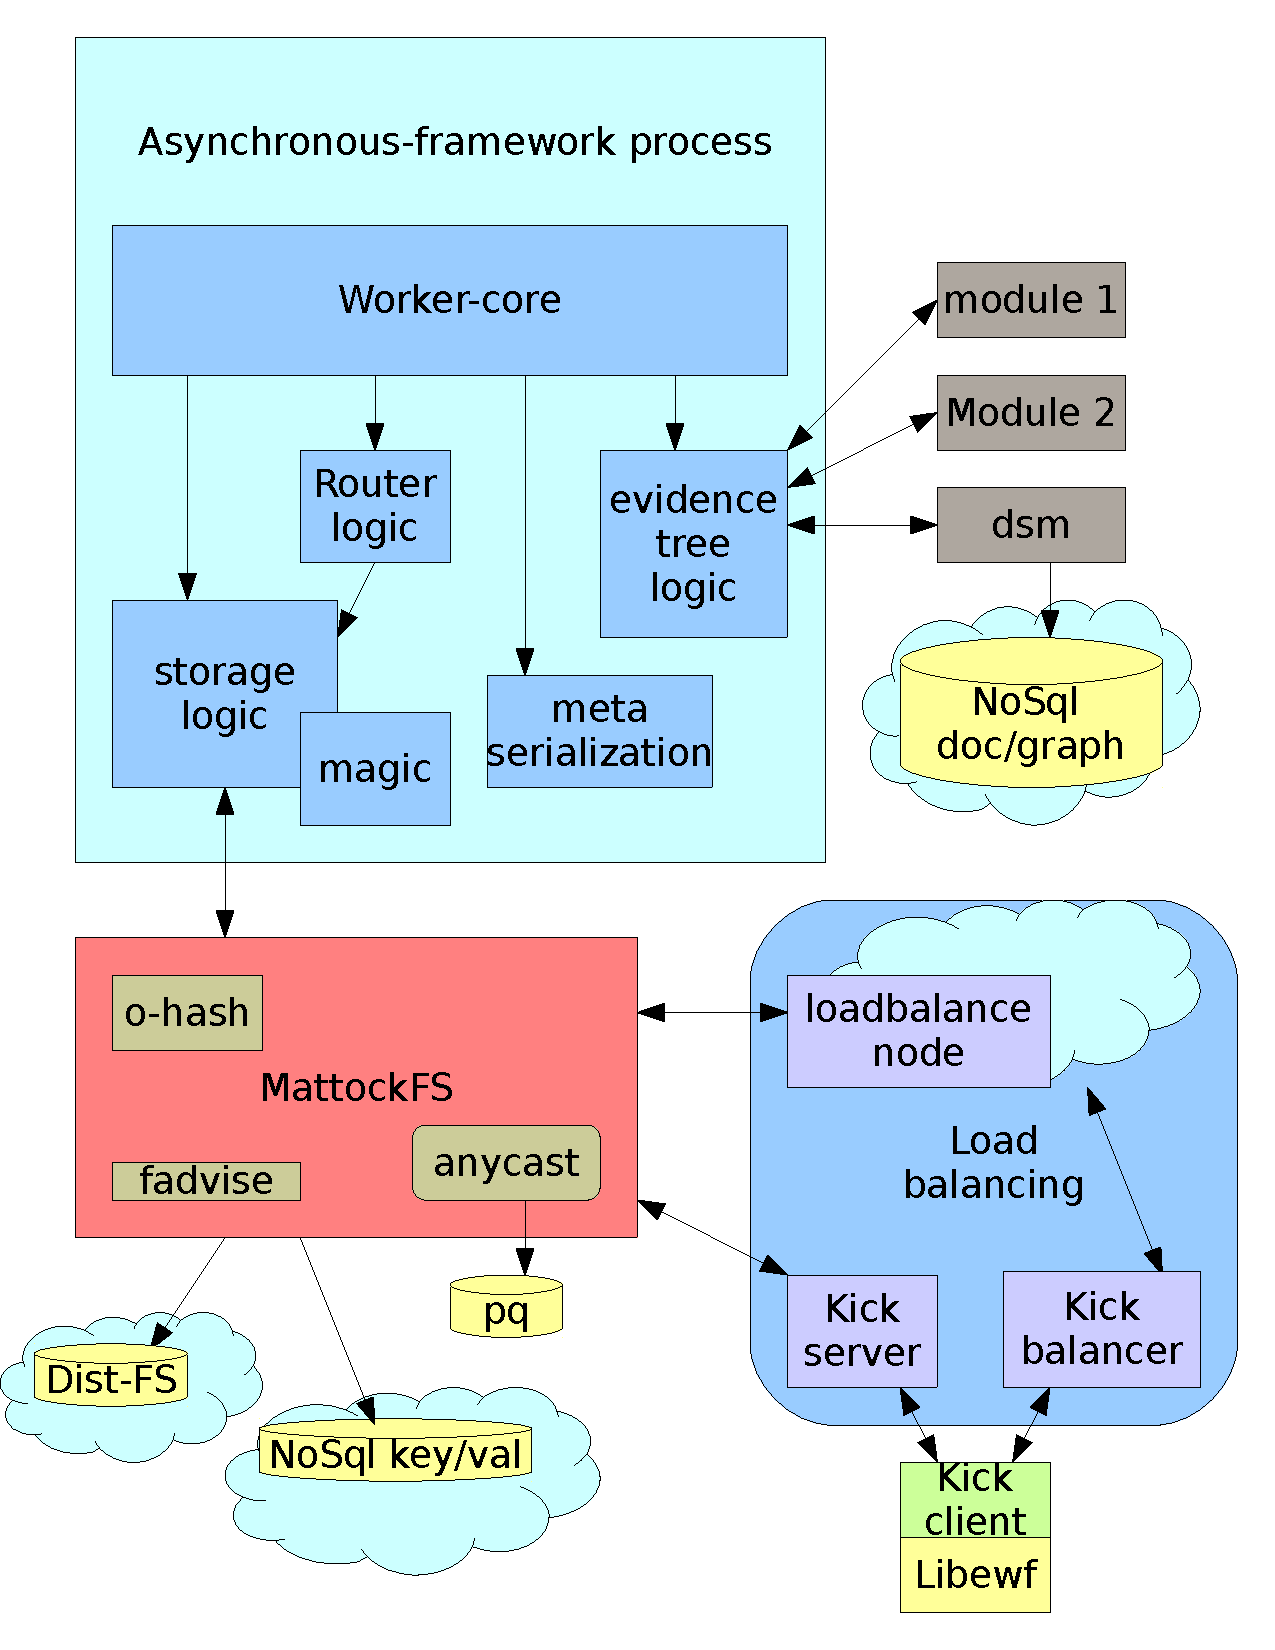
\includegraphics[width=100mm]{mattock/libraryviewmattock.pdf}
\caption{The base Mattock architecture}
\label{fig:FlowInOut}
\end{figure}
\subsection{The distributed long-path store}
The use of CarvPath annotations works very well for most data entities originating from digital media. In some cases, such as for log files on busy servers or large files downloaded in parallel over slow P2P connections, the files can be so fragmented that the CarvPath ends up being longer than what would be useful as a file or directory name in a file-system. To overcome that problem, long CarvPath annotations are replaced with a secure hash of the actual CarvPath. Given that storage tokens should be the same on each server node, knowledge to resolve these short notations back to their full CarvPath needs to be distributed. Given that the data stored are just simple key/value pairs, we propose that a NoSQL key/value store database technology would be most suitable to fill this task. A solution like Redis could be a viable implementation, but consideration regarding the speed versus persistence trade-off is important.
\subsection{SNFS vs distributed storage}
OCFA as used in its setup at the Dutch national police made use of SNFS on shared central block storage over fiber-channel. Alternative setups used a combination of local storage with NFS. It makes sense to set up a cluster of servers in such a way that kick-starting goes to a piece of local storage that is available on all other nodes using NFS mounts. A solution like that is basically the simplest form of non-redundant distributed storage. Mattock should work on these solutions or on any distributed storage system that allows for the creation of and efficient random access to relatively large \emph{sparse} data files. Distributed storage that emphasizes redundancy over performance might pose a problem, yet today technologies such as erasure encoding should allow for RAID-like properties for distributed storage that for larger numbers of nodes combine good performance with decent redundancy. Further study into suitable distributed storage solutions seems appropriate.
\subsection{MattockFS}
MattockFS is discussed in full detail in the main paper. It is a user-space file-system that is centered around CarvPath annotations and entities that consist of fragments and/or sparse regions. MattockFS runs on top of a distributed storage solution as described above and uses the distributed long-path store to store longer CarvPath annotations and make these work transparently on other nodes. The file-system provides the different async-modules with a file-system based API to storage and messaging. Apart from the CarvPath based data access, the MattockFS file-system based API provides:
\begin{itemize}
\item Immutability: The file-system provides facilities to create entities that are mutable only on creation.
\item CarvPath based batches that aim to provide for opportunistic hashes. A CarvPath can be marked as a batch and as it (and possibly its (ancestors or descendants) passes multiple modules before the batch is decommissioned, a hash may be calculated opportunistically.
\item Batch based fadvice: as batches get created and decommissioned, MattockFS can communicate with the kernel about chunks of repository data being potentially needed or will never get read again. The kernel should be able to use this data to become smarter with respect to page-cache usage, thus reducing the potential for page-cache miss performance issues.
\item Throttling: As the file-system keeps track of all active batches and notifies the kernel about data chunks no longer needed in the page-cache, MattockFS can provide statistics to async-modules that act as throttling advice for these modules. It provides total batches-size information and provides a \emph{what-if} facility allowing a module to query how much a new CarvPath would grow the active batches volume. An async-module should use this info to temporarily restrain from entering new (derived) data or uncached CarvPaths into the system until the point when the total amount of active batch space has gone down. 
\item AnyCast inter-process data exchange: Using extended attributes, symlinks and special directories, the file-system provides the possibility to mark data with a \emph{next} marker, placing it in an AnyCast like queue. It also allows to accept data for processing as a module.
\item Sparse capabilities: For processing a job and for one-time mutable access to a newly created data entity, the file-system provides sparse capabilities. These are basically one-time passwords for small chunks of authority. one-time passwords that can however be communicated between processes so that tool invocations by modules remains a possibility.
\item Total page-cache pressure: Provides the AnyCast monitor with info needed to potentially migrate jobs to other nodes.
\end{itemize}
\subsection{The AnyCast load-balance mesh-up}
Migrating a batch to an other node is expensive. Any opportunistic hashing will need to start from nothing, data won't exist in page cache on the other node, and unless the storage was highly redundant is the extra networking overhead of making the data available at all on the other node. For CPU intensive modules however, migrating a job might be well worth the cost. An AnyCast monitor process tries to keep track of things. The amount of page-cache potentially used up by active batches, the overall system load, the CPU and RAM usage of different worker modules, etc. This info is than all shared with AnyCast monitors on other server nodes. If a large imbalance is detected between node's, an AnyCast monitor may act as one or more modules and accept jobs and close their corresponding batches on the source server node. These jobs are than recreated by a monitor on a different node where they should normally live to complete the rest of the batch.
\subsection{Client/Server kick-starting}
With processing being done on a server or a cluster of AnyCast load-balance connected nodes, and with forensic disk images normally coming in on external media, entering the evidence data from the field into the lab-cluster is of main concern. Avoiding spurious image copying and load-balancing will seriously reduce the total processing time of large amounts of disk images on a distributed processing environment. To avoid spurious disk image copying, we define a per MattockFS-file-system instance network kick-start-server that accept data from a client side forensic disk image processing client. This means the whole of the image data will only be copied once, directly into a MattockFS repository. In order to avoid spurious load-balancing actions being needed, getting the client to send its disk image data to one of the the least loaded of the processing cluster is important. To allow this to happen, a per-cluster kick-start balancing server is defined. When a kick-start server starts up, it registers with the kick-start balancing server. The kick-start balancing server is part of the AnyCast balancing mesh-up network and is kept informed on system and page-cache load for each of the nodes. When a client wants to upload an image, it communicates this with the kick-start balancing server and is sent the network address and port of the kick-start server where it is expected to deliver its data. With such a construct, kick-starting will be relatively evenly spread amongst the server nodes.
\subsection{Module framework embedded lib-magic functionality}
In OCFA the libmagic file-type testing functionality was placed in a regular module. As we identified in Appendix A, this module would in most cases where the mime-type of the data was unknown be invoked as first and often last module for a batch. We identify that libmagic functionality is so common that it is warranted to make libmagic functionality part of the module framework.
\subsection{Distributed statefull routing logic}
In OCFA, the router module tended to be a processing bottleneck. For OCFA, lacking proper throttling facilities, this bottleneck turned out to actually mitigate the effects of the lack of throttling, but in a new architecture with solid throttling support, such bottleneck is undesirable. We pose that routing functionality can easily be distributed amongst the modules and be made an intrinsic part of the module framework. The FIVES project produced an alternate OCFA router that, other than the OCFA router was statefull in its rule-list processing. The use of such statefullness, combined with the availability of module generated meta-data, makes that the amount of meta-data exchanged between individual modules, in most cases can be limited to just two values:
\begin{itemize}
\item A router state string, allowing router logic inside of one module to continue the rule list where the previous module left of.
\item The data mime-type, allowing a module that is able to process multiple mime-types to distinguish between its types of input.
\end{itemize}
This choice makes it easy to quickly forward any other module generated meta-data blob to a default data-store module (DSM). So other than in OCFA where a mutable meta-data trace file was forwarded between all modules in a batch, in the Mattock architecture the per-module meta-data is stored as a derived-data MattockFS blob (with mime-type x-mattock/ENCODING; where ENCODING could be any serialization format identification) that is than immutable and is immediately forwarded to the DSM.  
\subsection{From SQL to graph and/or document based NoSQL}
We have already eliminated the use of SQL-server dependencies from most of the architecture. The module framework only has MattockFS as dependency, and MattockFS only uses an in-memory \emph{distributed} key/value store NoSQL database for a small part of its annotations. The data storage module however needs some place to store all meta-data in such a way that it becomes suitable both for use in a front-end system by investigators and for advanced querying by investigative-analyst/digital-investigator duos. Experience with investigative-analyst/digital-investigator duos and the use of OCFA databases has shown that most advanced queries tend to be exactly those queries that would translate to much more efficient and easy queries if the data had been modeled into a graph of vertexes and edges. Next to that, OCFA used XML blobs combined with specific indexed fields for much of its basic front-end related data storage. A task much more suitable for document databases. We suggest that taking these two distinct use-cases, a database technology used by Mattock should most likely opt to choose either graph or document oriented NoSQL technology over traditional SQL servers. Further, the chosen database technology preferably should be distributed. A quick market scan has revealed ArangoDb to possess all three desired qualities. ArangoDb is a distributed hybrid-model database that supports document and graph operations alike. More research is however needed to pick the most suitable database technology for Mattock.
\subsection{Using language-native asynchronous frameworks for the module framework}
When we look at the sizeable code-base of the OCFA framework, we can identify that more than a major part of the code-base is made up by the implementation of a custom asynchronous framework and a custom messaging bus. Where MattockFS mostly does away with the need for a custom messaging bus as it abstracts away the message bus with a file-system layer, the further need for a custom asynchronous framework has fully disappeared. NodeJS has mainstreamed language-specific asynchronous frameworks, and choosing for example Twisted for a Python based implementation of the module framework would take away much of the implementation time of such a module framework. The remaining per-language module framework would only need to implement:
\begin{itemize}
\item Communication with MattockFS according to the filesystem  based API that that system provides.
\item Throttling.
\item Use of a libmagic library for the given language as to determine mime-types of unidentified data.
\item Distributed statefull rule-list processing to set the next module for a batch.
\item An evidence tree API for implementing modules in a given language and the throttled evidence tree tree-walking logic.
\end{itemize}
\subsection{A single tree-graph, lambda and asynchronous operation oriented API}
OCFA had multiple APIs for making a module. The historic API was quite simple, but less suitable for deriving deep hierarchies from a single source. The newer tree-graph API was a bit more complex but also powerful enough to allow meta-data to be added to entities at each level of the tree. Given that a tree-graph API can be used to express each type of module, even simple ones, it is suggested that the Mattock module framework API be inspired by the OCFA tree-graph API. Given modern developments in programming languages that support a more functional higher order approach to programming. A modern API should probably leverage these developments and move away from a mostly object oriented approach to a more lambda oriented API. The creation of such an API should be subject of further study.
\section{Possible Mattock subjects for dissertations}
In the previous sections we described the outlines for a possible future academics geared open source computer forensic framework that could succeed OCFA and the Sleuthkit Hadoop framework. There is however quite a bit of research and development needed to eventually realize such a scalable framework in all its aspects. This document was written as an appendix to a paper on a core MattockFS system that focusses on the disk-cache and access control related aspects of the MattockFS subsystem. It would be very interesting if this document could be communicated with other students who are having problems picking a research topic for their dissertation. This section will list some important topics. It is thought that depending on the skills and knowledge of the student and the specific weight of the topic, a single , or at most two of these topics may constitute an amount of work suitable as outline for a research project.
\begin{figure}
\centering
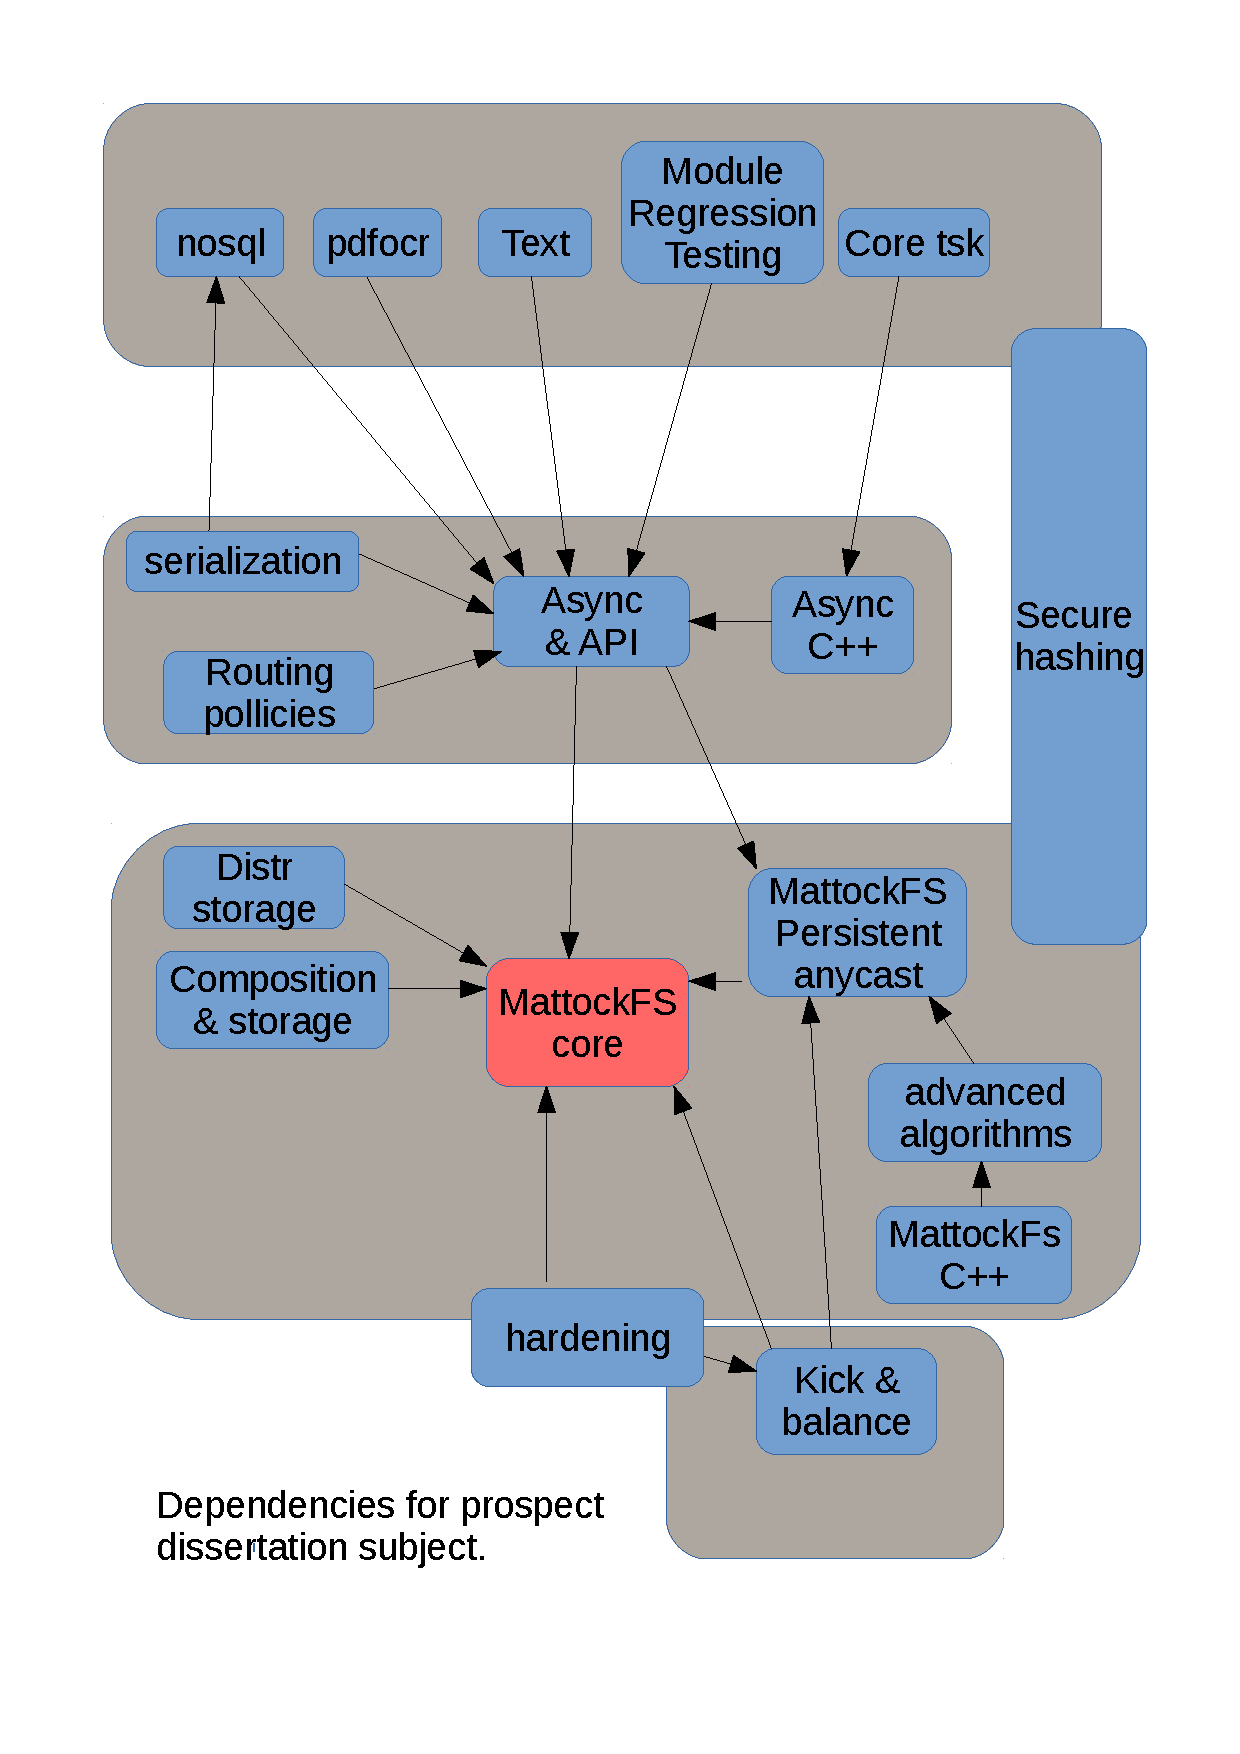
\includegraphics[width=100mm]{mattock/future.pdf}
\caption{Dependencies for prospect dissertation subjects.}
\label{fig:FlowInOut}
\end{figure}
\subsection{MattockFS related subjects}
While the core MattockFS system provides a demonstration of the page-cache, opportunistic hashing and access control aspects of this forensic computing geared user-space filesystem, the end result is not enough to power Mattock. Next to that there are some interesting enhancement related research topics that could form interesting research topics.
\subsubsection{Persistent AnyCast and long-path storage}
The MattockFS core defines the file-system based API for an embedded AnyCast. It does however not implement a persistent and of adequate performance 
AnyCast concept that works with the other MattockFS functionality. A final version of MattockFS should support transactional and persistent AnyCast operations. It should do this in such a way that it prioritizes jobs for a module according to the most disk-cache and opportunistic hashing friendly policy. Further the MattockFS core project does not address the subject of persistent distributed storage of long-paths. it provides a hook in its code, but allowing both technology that works for single-node persistence (for example Berkeley-dB) and technology that has better scaling properties (for example Redis) is not part of the initial implementation. 
This is the most pressing research topic as it will a first fully functional version of MattockFS, opening up more potential research topics.
\subsubsection{Advanced algorithms}
Once the first fully functional MattockFS is complete, it should become possible to experiment with multiple advanced algorithms. Things like additional unsolicited reads for opportunistic hashing, invocation of readahead and incore, per-target-module input and output throttling and many other strategies can be tested and benchmarked to create a set of CarvPath entity based algorithms for page-cache usage optimization, opportunistic hashing and AnyCast prioritization.
\subsubsection{MattockFS in C++}
Where Python is ideal for prototyping of systems like MattockFS, MattockFS is a very much pivotal aspect of Mattock where performance is concerned. Porting MattockFS to C++ and identifying and addressing performance bottlenecks is important if Mattock is to be used outside of o a purely academic setting.
\subsubsection{Hardening (part 1)}
While MattockFS addresses part of the access control needs for proper privilege separation and overall system robustness, there are aspects fundamental to the Linux operating system environments that don't work seamlessly when access control paradigms are concerned. Mandatory Access control systems such as SELinux and AppArmor provide the possibility to fill the security gaps that Linux leaves open by default in such a way that, together with firewall configurations, a hardened server would effectively confine untrusted modules to the tasks they were expected to do.
\subsubsection{Composition \& Storage}
While MattockFS and AFF4 on some parts overlap and in other parts conflict in their efforts, there are aspects to AFF4 that are unaddressed in the design and implementation of MattockFS. One important aspect that AFF4 propagates is the use of composed storage. Looking at if and how these composition principles presented with AFF4 could be made applicable for MattockFS without compromising on the core access-efficiency properties should make for an interesting research topic.
\subsubsection{Distributed storage}
OCFA used either centralized SNFS based storage or a setup-intensive NSF/local-storage mesh-up as underlying storage infrastructure for CarvFS data. The Sleuthkit Hadoop framework used HDFS. Each of these solutions comes with its own advantages and disadvantages. There has been much movement on the big-data front with regards to distributed storage. Erasure encoding and other RAID like technologies seem to enable a middle ground between the desire for import performance and the desire for robust redundant storage. Access control is also an important aspect of any distributed storage solution. Looking into the available technology and determining the one(s) most suitable to use as storage basis for MattockFS should make for an interesting research topic. 
\subsection{Kick \& Balance}
MattockFS as a service i meant to be a local service only. Communication with MattockFS and the creation of a distributed processing cluster is done by a networked kick-starting and balancing system.
\subsubsection{Load-balancing}
At the core of the kick-starting and balancing system is the AnyCast load-balancing mesh-up. The nodes of this mesh-up monitor individual MattockFS instances and server loads and determine what batches should be migrated to less busy nodes. Given the intrinsic cost of migration, algorithms for migration should be constructed very carefully and should be meticulously profiled before deciding on the most suitable algorithm.  Creation of these algorithms and the mesh-up that uses them should provide for quite a challenging research topic.
\subsubsection{Kick-starting}
The kick-starting system couples forensic investigator workstations with both the load balancing system and MattockFS. The client needs to decode the forensic disk images (for example using LibEWF and/or LibAFF) and send the potentially sparse data in an efficient way to the kick-start server that will hand it to MattockFS for further processing. The client needs to be able to find a kick-start balancer on the network that is acting on behalf of the proper investigation. Design and implementation of these kick-starting related subsystems should provide for an interesting research topic.
\subsubsection{Hardening (part 2)}
Next to the hardening with firewall rules and mandatory access controls, we must also consider the inter-node communication to be potentially vulnerable to undesirable unauthorized access. As part of the hardening, looking at protecting the communication and providing authorization tokens and encryption in our communications should be considered an important aspect of the hardening of our Mattock architecture.
\subsection{Module Framework related subjects}
\subsubsection{Asynchronous framework \& tree-graph API}
The initial definition of a modern tree-graph module API and base framework implementation in most likely Python should together with a completely functional MattockFS create the first (at least locally) working version of a Mattock architecture. The first version could implement mostly static and/or hard-coded routing and use any type of serialization. The focus should be on interacting both with the throttling facilities of MattockFS and with a tree-graph-API based module. The design and implementation of this initial module framework should make a challenging topic.
\subsubsection{Serialization}
Where OCFA used XML for its meta data serialization, XML in its processing is relatively expensive. There are other interesting meta-data serialization issues such as how to serialize timestamps from different time sources. Further, the chosen database technology might also be relevant to the serialization used. Should we serialize in a way that represents our central data model or in a way that best fits the tool or library functionality our module if wrapping. This is a quite open but yet essential research topic. 
\subsubsection{Routing policies}
The FIVES project created the concept of a statefull rule-list traversal. Mattock requires a distributed version of that. Given that a module knows the module it is, only part of the rule-list is relevant to it. this research project should look at the possibilities of creating a distributed per-module \emph{next hop} FIVES router.
\subsubsection{Asynchronous framework \& C++}
While most of the computer forensics modules should be easy and most convenient to create in Python, the framework would not be complete without an efficient implementation of disk-image and file-system analysis modules. Given the availability of libraries, and the performance of C++ when compared to Python, it is desirable that these specific modules, especially modules based on the Sleuthkit library (libtsk) can be implemented in C++.  
\subsection{Module related subjects}
\subsubsection{Module regression testing}
As identified by Garfinkel (Garfinkel 2010), OCFA did not address all the scaling needs of academics in the fields of digital forensics. The most major shortcoming was the inability of the OCFA architecture to allow for small scale setup and module regression analysis. As MattockFS and the module framework should not require the minimal scaling properties of OCFA, the small setup should already be covered. Yet the creation of a same-interface module regression testing filesystem and/or same interface regression-testing tree-walk tool, could provide for an environment that would allow regression analysis at different scaling levels.
\subsubsection{Core libtsk modules}
While framework in important, without filesystem and disk layout modules the framework itself does not constitute a digital forensics framework. We need these modules and the Sleuthkit library provides the facilities for creating these modules. OCFA has implementations of several libtsk based modules that could serve as guide in creating similar modules for Mattock. The creation of these core modules should provide for an interesting research topic and should, should promote Mattock from being a data processing framework to being a digital forensic framework.
\subsubsection{DSM \& NoSQL}
While we already know that centralized SQL technology is poorly suited as central meta-data store, there is a lot that needs to be researched. What database technology \emph{is} most suitable? Should we run the database nodes on the same servers we run our Mattock servers on? Can we get away with single model storage or are the different use cases so different that we need to simultaneously store our data in different models, maybe even different database technologies. What database front-end options are there for querying our data? Answering these questions and developing a data store module and basic database front-end according to these answers should make for a rewarding research topic.
\subsubsection{Text extraction and indexing}
A second set of important modules for a forensic framework are modules related to making the corpus searchable with text. To do this we need to develop or port text extraction modules. OCFA comes with some basic text extraction modules such as text extraction from pdf, word, word-perfect, mime and sqlite. Many more should be possible, but that is less interesting. The interesting research topic lies in combining these modules with an indexing module that plays nice with the distributed processing concept. Selecting indexing technology that allows bottleneck free distributed indexing and efficient querying from some front-end. This research project should aim to provide one or two simple text extraction modules, an indexing module and a simple index querying front-end.
\subsubsection{Pdf \& OCR}
Until now, most module functionality described was just a reimplementation of what was already available in some form in legacy frameworks like OCFA, fitted to scale to a more decentralized bottleneck-free distributed processing environment. This subject goes a few steps further than that. Apart from architectural flaws, OCFA performance occasionally suffered from a more module related flaw. The performance of OCR on mixed-orientation scanned document PDFs. The implementation of a sufficiently performing solution for PDF-OCR will stress mattock to its fullest. PDF-OCR jobs are possibly the most CPU processing intensive jobs in a forensic processing tool-chain. The occurrence of scanned document PDFs is also something that is very much bulky. A 100 disk image investigation may have just one or two disk images that hold many thousands of scanned document PDFs, making Mattock's load balancing facilities truly proof themselves. But even with load balancing working full gear, there are other inefficiencies in mixed-orientation scanned document OCR that should proof quite a challenge. 
\subsection{Secure hashing}
It isn't really Mattock specific, but as addressed in a different appendix, both SHA1 and MD5 are deprecated and risky secure hashing algorithms. To continue to use in forensic frameworks for compatibility reasons is not without its risks. Solid research in providing a migrational path with Mattock and with commonly used hash sets like Virusshare, national child pornography databases and NSRL seems to be of major importance.
\section{Conclusion}
While MattockFS core provides proof of the possibility to leverage the power of CarvPath entities as basis for a disk-cache efficient privilege separated forensic framework, the implementation of a whole framework that is usable in both an academic setting and for full scale investigations will require quite some additional research. This appendix sketched the outlines of such a framework and proposed a list of potential dissertation subjects for computer forensic M.Sc students struggling with finding a research topic. If this topic speaks to students, the combined effort may lead to a interesting open source framework that could power computer forensic research for years to come.

